% domain of integration for Compton scattering
\begin{center}
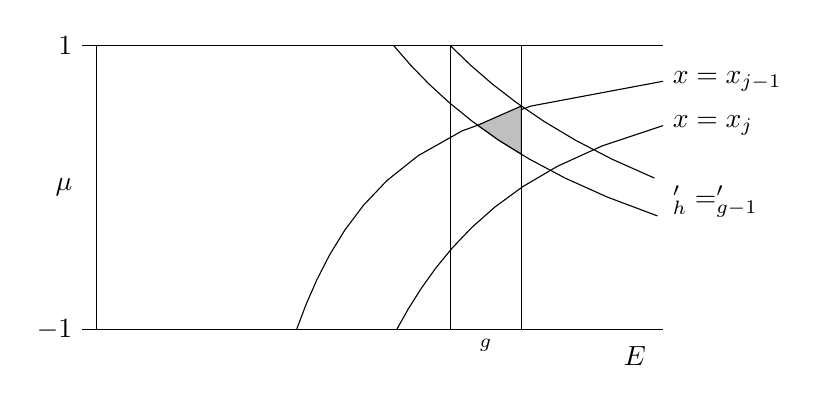
\begin{tikzpicture} [scale=1.8]
% the axes and quadrature box
  \draw(-0.1, -1) -- (4, -1);
  \draw(0, -1) -- (0, 1);
  \draw(-0.1, 1) -- (4, 1);
  \draw(2.5, -1) -- (2.5, 1);
  \draw(3, -1) -- (3, 1);
% x = constant curves
% E' = 2/sqrt{1 - mu}
\draw( 1.4142 , -1.0 ) --
( 1.4805 , -0.825 ) --
( 1.557 , -0.65 ) --
( 1.6468 , -0.475 ) --
( 1.7541 , -0.3 ) --
( 1.8856, -0.125 ) --
( 2.052 , 0.05 ) --
( 2.2718 , 0.225 ) --
( 2.582 , 0.4 ) --
( 3.0679, 0.575 ) --
( 4.0 , 0.75 );
% E' = 3/sqrt{1 - mu}
\draw( 2.1213 , -1.0 ) --
( 2.2019 , -0.85625 ) --
( 2.2925, -0.7125 ) --
( 2.3952 , -0.56875 ) --
( 2.5131 , -0.425 ) --
( 2.6504 , -0.28125 ) --
( 2.8128 , -0.1375 ) --
( 3.0094 , 0.00625 ) --
( 3.254 , 0.15 ) --
( 3.5698 , 0.29375 ) --
( 4.0 , 0.4375 );
% outgoing energy bin
\draw( 3.9388, 0.0667 ) --
( 3.6396, 0.2 ) --
( 3.3826 , 0.3333 ) --
( 3.1595 , 0.4667 ) --
( 2.9640 , 0.6 ) --
( 2.7913 , 0.7333 ) --
( 2.6376, 0.8667 ) --
( 2.5 , 1.0 );
\draw( 3.9598, -0.2 ) --
( 3.6050, -0.06667 ) --
( 3.3086, 0.06667 ) --
( 3.0573, 0.2 ) --
( 2.8414 , 0.3333 ) --
( 2.654, 0.4667 ) --
( 2.4898, 0.6 ) --
( 2.3447 , 0.7333 ) --
( 2.2156, 0.8667 ) --
( 2.1 , 1.0 );
% quadrature region
\filldraw[fill = gray!50]  (2.6920, 0.4396) --
(3.0000, 0.5755) --
(3.0000, 0.2354) --
(2.8414 , 0.3333 ) -- cycle;
% labels
  \node[left] at(-0.1, -1){$-1$};
  \node[left]  at(-0.1, 1){$1$};
  \node[left]  at(-0.1, 0){$\mu$};
  \node[below] at(2.75, -1){$\calE_g$};
  \node[below]  at(3.8, -1.05){$E$};
  \node[right] at(4, 0.75){$x = x_{j-1}$};
  \node[right]  at(4, 0.4375){$x = x_j$};
  \node[right]  at(4, -0.1){$\calE'_h = \calE'_{g-1}$};
\end{tikzpicture}
\caption{Domain of integration for Compton scattering}
\label{Fig:Compton}
\end{center} 
